\documentclass[]{elsarticle} %review=doublespace preprint=single 5p=2 column
%DIF LATEXDIFF DIFFERENCE FILE
%DIF DEL R0-Density-Reanalysis-v0.tex   Wed Sep 15 22:11:11 2021
%DIF ADD R0-Density-Reanalysis.tex      Wed Sep 15 22:10:06 2021
%%% Begin My package additions %%%%%%%%%%%%%%%%%%%
\usepackage[hyphens]{url}

  \journal{Geographical Analysis} % Sets Journal name


\usepackage{lineno} % add
  \linenumbers % turns line numbering on
\providecommand{\tightlist}{%
  \setlength{\itemsep}{0pt}\setlength{\parskip}{0pt}}

\usepackage{graphicx}
\usepackage{booktabs} % book-quality tables
%%%%%%%%%%%%%%%% end my additions to header

\usepackage[T1]{fontenc}
\usepackage{lmodern}
\usepackage{amssymb,amsmath}
\usepackage{ifxetex,ifluatex}
\usepackage{fixltx2e} % provides \textsubscript
% use upquote if available, for straight quotes in verbatim environments
\IfFileExists{upquote.sty}{\usepackage{upquote}}{}
\ifnum 0\ifxetex 1\fi\ifluatex 1\fi=0 % if pdftex
  \usepackage[utf8]{inputenc}
\else % if luatex or xelatex
  \usepackage{fontspec}
  \ifxetex
    \usepackage{xltxtra,xunicode}
  \fi
  \defaultfontfeatures{Mapping=tex-text,Scale=MatchLowercase}
  \newcommand{\euro}{€}
\fi
% use microtype if available
\IfFileExists{microtype.sty}{\usepackage{microtype}}{}
\bibliographystyle{elsarticle-harv}
\ifxetex
  \usepackage[setpagesize=false, % page size defined by xetex
              unicode=false, % unicode breaks when used with xetex
              xetex]{hyperref}
\else
  \usepackage[unicode=true]{hyperref}
\fi
\hypersetup{breaklinks=true,
            bookmarks=true,
            pdfauthor={},
            pdftitle={Reproducibility of research during COVID-19: examining the case of population density and the basic reproductive rate from the perspective of spatial analysis},
            colorlinks=false,
            urlcolor=blue,
            linkcolor=magenta,
            pdfborder={0 0 0}}
\urlstyle{same}  % don't use monospace font for urls

\setcounter{secnumdepth}{0}
% Pandoc toggle for numbering sections (defaults to be off)
\setcounter{secnumdepth}{0}

% Pandoc citation processing
%DIF 59-60d59
%DIF < \newlength{\csllabelwidth}
%DIF < \setlength{\csllabelwidth}{3em}
%DIF -------
\newlength{\cslhangindent}
\setlength{\cslhangindent}{1.5em}
%DIF 63a61-62
\newlength{\csllabelwidth} %DIF > 
\setlength{\csllabelwidth}{3em} %DIF > 
%DIF -------
% for Pandoc 2.8 to 2.10.1
\newenvironment{cslreferences}%
  {}%
  {\par}
% For Pandoc 2.11+
%DIF 68c68
%DIF < \newenvironment{CSLReferences}[3] % #1 hanging-ident, #2 entry spacing
%DIF -------
\newenvironment{CSLReferences}[2] % #1 hanging-ident, #2 entry spacing %DIF > 
%DIF -------
 {% don't indent paragraphs
  \setlength{\parindent}{0pt}
  % turn on hanging indent if param 1 is 1
  \ifodd #1 \everypar{\setlength{\hangindent}{\cslhangindent}}\ignorespaces\fi
  % set entry spacing
  \ifnum #2 > 0
  \setlength{\parskip}{#2\baselineskip}
  \fi
 }%
 {}
%DIF 79c79
%DIF < \usepackage{calc} % for calculating minipage widths
%DIF -------
\usepackage{calc} %DIF > 
%DIF -------
\newcommand{\CSLBlock}[1]{#1\hfill\break}
\newcommand{\CSLLeftMargin}[1]{\parbox[t]{\csllabelwidth}{#1}}
%DIF 82c82
%DIF < \newcommand{\CSLRightInline}[1]{\parbox[t]{\linewidth - \csllabelwidth}{#1}}
%DIF -------
\newcommand{\CSLRightInline}[1]{\parbox[t]{\linewidth - \csllabelwidth}{#1}\break} %DIF > 
%DIF -------
\newcommand{\CSLIndent}[1]{\hspace{\cslhangindent}#1}

% Pandoc header
\usepackage{setspace}\onehalfspacing
\usepackage{booktabs}
\usepackage{longtable}
\usepackage{array}
\usepackage{multirow}
\usepackage{wrapfig}
\usepackage{float}
\usepackage{colortbl}
\usepackage{pdflscape}
\usepackage{tabu}
\usepackage{threeparttable}
\usepackage{threeparttablex}
\usepackage[normalem]{ulem}
\usepackage{makecell}
\usepackage{xcolor}
%DIF PREAMBLE EXTENSION ADDED BY LATEXDIFF
%DIF UNDERLINE PREAMBLE %DIF PREAMBLE
\RequirePackage[normalem]{ulem} %DIF PREAMBLE
\RequirePackage{color}\definecolor{RED}{rgb}{1,0,0}\definecolor{BLUE}{rgb}{0,0,1} %DIF PREAMBLE
\providecommand{\DIFaddtex}[1]{{\protect\color{blue}\uwave{#1}}} %DIF PREAMBLE
\providecommand{\DIFdeltex}[1]{{\protect\color{red}\sout{#1}}}                      %DIF PREAMBLE
%DIF SAFE PREAMBLE %DIF PREAMBLE
\providecommand{\DIFaddbegin}{} %DIF PREAMBLE
\providecommand{\DIFaddend}{} %DIF PREAMBLE
\providecommand{\DIFdelbegin}{} %DIF PREAMBLE
\providecommand{\DIFdelend}{} %DIF PREAMBLE
\providecommand{\DIFmodbegin}{} %DIF PREAMBLE
\providecommand{\DIFmodend}{} %DIF PREAMBLE
%DIF FLOATSAFE PREAMBLE %DIF PREAMBLE
\providecommand{\DIFaddFL}[1]{\DIFadd{#1}} %DIF PREAMBLE
\providecommand{\DIFdelFL}[1]{\DIFdel{#1}} %DIF PREAMBLE
\providecommand{\DIFaddbeginFL}{} %DIF PREAMBLE
\providecommand{\DIFaddendFL}{} %DIF PREAMBLE
\providecommand{\DIFdelbeginFL}{} %DIF PREAMBLE
\providecommand{\DIFdelendFL}{} %DIF PREAMBLE
%DIF HYPERREF PREAMBLE %DIF PREAMBLE
\providecommand{\DIFadd}[1]{\texorpdfstring{\DIFaddtex{#1}}{#1}} %DIF PREAMBLE
\providecommand{\DIFdel}[1]{\texorpdfstring{\DIFdeltex{#1}}{}} %DIF PREAMBLE
\newcommand{\DIFscaledelfig}{0.5}
%DIF HIGHLIGHTGRAPHICS PREAMBLE %DIF PREAMBLE
\RequirePackage{settobox} %DIF PREAMBLE
\RequirePackage{letltxmacro} %DIF PREAMBLE
\newsavebox{\DIFdelgraphicsbox} %DIF PREAMBLE
\newlength{\DIFdelgraphicswidth} %DIF PREAMBLE
\newlength{\DIFdelgraphicsheight} %DIF PREAMBLE
% store original definition of \includegraphics %DIF PREAMBLE
\LetLtxMacro{\DIFOincludegraphics}{\includegraphics} %DIF PREAMBLE
\newcommand{\DIFaddincludegraphics}[2][]{{\color{blue}\fbox{\DIFOincludegraphics[#1]{#2}}}} %DIF PREAMBLE
\newcommand{\DIFdelincludegraphics}[2][]{% %DIF PREAMBLE
\sbox{\DIFdelgraphicsbox}{\DIFOincludegraphics[#1]{#2}}% %DIF PREAMBLE
\settoboxwidth{\DIFdelgraphicswidth}{\DIFdelgraphicsbox} %DIF PREAMBLE
\settoboxtotalheight{\DIFdelgraphicsheight}{\DIFdelgraphicsbox} %DIF PREAMBLE
\scalebox{\DIFscaledelfig}{% %DIF PREAMBLE
\parbox[b]{\DIFdelgraphicswidth}{\usebox{\DIFdelgraphicsbox}\\[-\baselineskip] \rule{\DIFdelgraphicswidth}{0em}}\llap{\resizebox{\DIFdelgraphicswidth}{\DIFdelgraphicsheight}{% %DIF PREAMBLE
\setlength{\unitlength}{\DIFdelgraphicswidth}% %DIF PREAMBLE
\begin{picture}(1,1)% %DIF PREAMBLE
\thicklines\linethickness{2pt} %DIF PREAMBLE
{\color[rgb]{1,0,0}\put(0,0){\framebox(1,1){}}}% %DIF PREAMBLE
{\color[rgb]{1,0,0}\put(0,0){\line( 1,1){1}}}% %DIF PREAMBLE
{\color[rgb]{1,0,0}\put(0,1){\line(1,-1){1}}}% %DIF PREAMBLE
\end{picture}% %DIF PREAMBLE
}\hspace*{3pt}}} %DIF PREAMBLE
} %DIF PREAMBLE
\LetLtxMacro{\DIFOaddbegin}{\DIFaddbegin} %DIF PREAMBLE
\LetLtxMacro{\DIFOaddend}{\DIFaddend} %DIF PREAMBLE
\LetLtxMacro{\DIFOdelbegin}{\DIFdelbegin} %DIF PREAMBLE
\LetLtxMacro{\DIFOdelend}{\DIFdelend} %DIF PREAMBLE
\DeclareRobustCommand{\DIFaddbegin}{\DIFOaddbegin \let\includegraphics\DIFaddincludegraphics} %DIF PREAMBLE
\DeclareRobustCommand{\DIFaddend}{\DIFOaddend \let\includegraphics\DIFOincludegraphics} %DIF PREAMBLE
\DeclareRobustCommand{\DIFdelbegin}{\DIFOdelbegin \let\includegraphics\DIFdelincludegraphics} %DIF PREAMBLE
\DeclareRobustCommand{\DIFdelend}{\DIFOaddend \let\includegraphics\DIFOincludegraphics} %DIF PREAMBLE
\LetLtxMacro{\DIFOaddbeginFL}{\DIFaddbeginFL} %DIF PREAMBLE
\LetLtxMacro{\DIFOaddendFL}{\DIFaddendFL} %DIF PREAMBLE
\LetLtxMacro{\DIFOdelbeginFL}{\DIFdelbeginFL} %DIF PREAMBLE
\LetLtxMacro{\DIFOdelendFL}{\DIFdelendFL} %DIF PREAMBLE
\DeclareRobustCommand{\DIFaddbeginFL}{\DIFOaddbeginFL \let\includegraphics\DIFaddincludegraphics} %DIF PREAMBLE
\DeclareRobustCommand{\DIFaddendFL}{\DIFOaddendFL \let\includegraphics\DIFOincludegraphics} %DIF PREAMBLE
\DeclareRobustCommand{\DIFdelbeginFL}{\DIFOdelbeginFL \let\includegraphics\DIFdelincludegraphics} %DIF PREAMBLE
\DeclareRobustCommand{\DIFdelendFL}{\DIFOaddendFL \let\includegraphics\DIFOincludegraphics} %DIF PREAMBLE
%DIF LISTINGS PREAMBLE %DIF PREAMBLE
\RequirePackage{listings} %DIF PREAMBLE
\RequirePackage{color} %DIF PREAMBLE
\lstdefinelanguage{DIFcode}{ %DIF PREAMBLE
%DIF DIFCODE_UNDERLINE %DIF PREAMBLE
  moredelim=[il][\color{red}\sout]{\%DIF\ <\ }, %DIF PREAMBLE
  moredelim=[il][\color{blue}\uwave]{\%DIF\ >\ } %DIF PREAMBLE
} %DIF PREAMBLE
\lstdefinestyle{DIFverbatimstyle}{ %DIF PREAMBLE
	language=DIFcode, %DIF PREAMBLE
	basicstyle=\ttfamily, %DIF PREAMBLE
	columns=fullflexible, %DIF PREAMBLE
	keepspaces=true %DIF PREAMBLE
} %DIF PREAMBLE
\lstnewenvironment{DIFverbatim}{\lstset{style=DIFverbatimstyle}}{} %DIF PREAMBLE
\lstnewenvironment{DIFverbatim*}{\lstset{style=DIFverbatimstyle,showspaces=true}}{} %DIF PREAMBLE
%DIF END PREAMBLE EXTENSION ADDED BY LATEXDIFF

\begin{document}
\begin{frontmatter}

  \title{Reproducibility of research during COVID-19: examining the case
of population density and the basic reproductive rate from the
perspective of spatial analysis}
    \author[University]{Author\corref{1}}
   \ead{author@institution.edu} 
      \address[University]{Department, Street, City, State ZIP}
      \cortext[1]{Corresponding Author}

  \begin{abstract}
  The emergence of the novel SARS-CoV-2 coronavirus and the global
  COVID-19 pandemic \DIFdelbegin \DIFdel{has }\DIFdelend \DIFaddbegin \DIFadd{in 2019 }\DIFaddend led to explosive growth in scientific
  research. Alas, much of the research in the literature lacks
  conditions to be reproducible, and recent publications on the
  association between population density and the basic reproductive
  number of SARS-CoV-2 are no exception. Relatively few papers share
  code and data sufficiently, which hinders not only verification but
  additional experimentation. In this paper, an example of reproducible
  research shows the potential of spatial analysis for epidemiology
  research during COVID-19. Transparency and openness means that
  independent researchers can, with \DIFdelbegin \DIFdel{relatively }\DIFdelend \DIFaddbegin \DIFadd{only }\DIFaddend modest efforts, verify findings
  and use different approaches as appropriate. Given the high stakes of
  the situation, it is essential that scientific findings, on which good
  policy depends, are as robust as possible; as the empirical example
  shows, reproducibility is one of the keys to ensure this.
  \end{abstract}

 \end{frontmatter}

\newpage

\hypertarget{introduction}{%
\section{Introduction}\label{introduction}}

The emergence of the novel SARS-CoV-2 coronavirus in 2019, and the
global pandemic that followed in its wake, led to an explosive growth of
research around the globe. According to Fraser et al. (2021), over
125,000 COVID-19-related papers were released in the first ten months
from the first confirmed case of the disease. Of these, more than 30,000
were shared in pre-print servers, the use of which also exploded in the
past year (Añazco et al., 2021; Kwon, 2020; Vlasschaert et al., 2020).

Given the ruinous human and economic cost of the pandemic, there has
been a natural tension in the scientific community between the need to
publish research results quickly and the imperative to maintain
consistently high quality standards in scientific reporting; indeed, a
call for maintaining the standards in published research \DIFdelbegin \DIFdel{has }\DIFdelend termed the
deluge of COVID-19 publications a ``carnage of substandard research''
(Bramstedt, 2020). Part of the challenge of maintaining quality
standards in published research is that, despite an abundance of
recommendations and guidelines (e.g., Broggini et al., 2017; Brunsdon
and Comber, 2020; Ince et al., 2012; Ioannidis et al., 2014), in
practice reproducibility has remained a lofty and somewhat aspirational
goal (Konkol et al., 2019; Konkol and Kray, 2019). As reported in the
literature, only a woefully small proportion of published research was
actually reproducible before the pandemic (Iqbal et al., 2016; Stodden
et al., 2018), and the situation does not appear to have changed
substantially since (Gustot, 2020; Sumner et al., 2020).

The push for open \DIFdelbegin \DIFdel{data and software , }\DIFdelend \DIFaddbegin \DIFadd{software and data (Arribas-Bel et al., 2021; e.g.,
Bivand, 2020), }\DIFaddend along with more strenuous efforts towards open,
reproducible research, is simply a continuation of long-standing
scientific practices of independent verification. Despite the (at times
disproportionate) attention that high profile scandals in science tend
to elicit in the media, science as a collective endeavor is remarkable
for being a self-correcting enterprise, one with built-in mechanisms and
incentives to weed out erroneous ideas. Over the long term, facts tend
to prevail in science. At stake is the shorter-term impacts that
research may have in other spheres of economic and social life. The case
of economists Reinhart and Rogoff comes to mind: by the time the
inaccuracies and errors in their research were uncovered (see Herndon et
al., 2014), their claims about debt and economic growth had already been
seized by policy-makers on both sides of the Atlantic to justify
austerity policies in the aftermath of the Great Recession of
2007-2009\footnote{Nobel Prize in Economics Paul Krugman noted that
  ``Reinhart--Rogoff may have had more immediate influence on public
  debate than any previous paper in the history of economics''
  \url{https://www.nybooks.com/articles/2013/06/06/how-case-austerity-has-crumbled/?pagination=false}}.
As later research has demonstrated, those policies cast a long shadow,
and their sequels continued to be felt for years (Basu et al., 2017).

In the context of COVID-19, a topic that has grabbed the imagination of
numerous thinkers has been the prospect of life in cities after the
pandemic (\DIFaddbegin \DIFadd{e.g., }\DIFaddend Florida et al., 2020); \DIFaddbegin \DIFadd{as a result, }\DIFaddend the implications of
the pandemic for urban planning, design, and management are the topic of
ongoing research (\DIFaddbegin \DIFadd{e.g., }\DIFaddend Sharifi and Khavarian-Garmsir, 2020). The fact
that the worst of the pandemic was initially felt in dense population
centers such as Wuhan, Milan, Madrid, and New York, unleashed a torrent
of research into the associations between density and the spread of the
pandemic. \DIFdelbegin \DIFdel{he }\DIFdelend \DIFaddbegin \DIFadd{The }\DIFaddend answers to some important questions hang on the results of
these research efforts. For example, are lower density regions safer
from the pandemic? Are de-densification policies warranted, even if just
in the short term? \DIFdelbegin \DIFdel{And in }\DIFdelend \DIFaddbegin \DIFadd{In }\DIFaddend the longer term, will the risks of life in high
density regions presage a flight from cities? \DIFdelbegin \DIFdel{What }\DIFdelend \DIFaddbegin \DIFadd{And, what }\DIFaddend are the
implications of the pandemic for future urban planning and practice?
Over the past year, numerous papers have sought to throw light on the
underlying issue of density and the pandemic; nonetheless the results,
as will be detailed next, remain mixed. Further, to complicate matters,
precious few of these studies appear to be sufficiently open to support
independent verification.

The objective of this paper is to illustrate the importance of
reproducibility in research in the context of the flood of COVID-19
papers. \DIFdelbegin \DIFdel{To thisend, }\DIFdelend \DIFaddbegin \DIFadd{For this, I focus on }\DIFaddend a recent study by Sy et al. (2021) \DIFdelbegin \DIFdel{is chosen as an
example of }\DIFdelend \DIFaddbegin \DIFadd{that
examined the correlation between the basic reproductive number of
COVID-19, \(R_0\), and population density. The basic reproductive number
is a summary measure of contact rates, probability of transmission of a
pathogen, and duration of infectiousness. In rough terms, it measures
how many new infections each infections begets. The paper of Sy et al.
(2021) was selected for being, in the literature examined, almost alone
in supporting }\DIFaddend reproducible research. \DIFdelbegin \DIFdel{The objective }\DIFdelend \DIFaddbegin \DIFadd{Accordingly, I wish to be clear
that my objective in singling their work for discussion }\DIFaddend is not to malign
\DIFdelbegin \DIFdel{the
analysis of these researchers}\DIFdelend \DIFaddbegin \DIFadd{their efforts}\DIFaddend , but rather to demonstrate \DIFdelbegin \DIFdel{the value of
openness to allow for independent verification and further analysis. Open }\DIFdelend \DIFaddbegin \DIFadd{how open and reproducible
research efforts can greatly help to accelerate discovery. More
concretely, open }\DIFaddend data and open code mean that an independent researcher
can, with only modest efforts, not only verify the findings reported,
but also examine the same data from a perspective which may not have
been available to the original researchers due to differences in
disciplinary perspectives, methodological traditions, and/or training,
among other possible factors. The example, which shows consequential
changes in the conclusions reached by different analyses, should serve
as a call to researchers to redouble their efforts to increase
transparency and reproducibility in \DIFdelbegin \DIFdel{research. The present paper , in addition, }\DIFdelend \DIFaddbegin \DIFadd{their research. In this spirit, the
present paper also }\DIFaddend aims to show how data can be packaged in
well-documented, shareable units, and code can be embedded into
self-contained documents suitable for review and independent
verification. The source for this paper is an
\href{http://rmarkdown.rstudio.com}{R Markdown} document which, along
with the data package, will be available in a public
repository\footnote{For peer-review purposes, the data package and code
  are currently in an anonymous Drive folder:
  \url{https://drive.google.com/drive/folders/1cT6tcUc1pJ4aT5ajQ0emO0lyS46P8Ige?usp=sharing}}.

\hypertarget{background-the-intuitive-relationship-between-density-and-spread-of-contagious-diseases}{%
\section{Background: the intuitive relationship between density and
spread of contagious
diseases}\label{background-the-intuitive-relationship-between-density-and-spread-of-contagious-diseases}}

The concern with population density and the spread of the virus during
the COVID-19 pandemic was fueled, at least in part, by dramatic scenes
seen in real-time around the world from large urban centers such as
Wuhan, Milan, Madrid, and New York. In theory, there are good reasons to
believe that higher density \DIFdelbegin \DIFdel{may }\DIFdelend \DIFaddbegin \DIFadd{could }\DIFaddend have a positive association with the
transmission of a contagious virus. It has long been known that the
potential for inter-personal contact is greater in regions with higher
density (see for example the research on urban fields and
time-geography, including Farber and Páez, 2011; Moore, 1970; Moore and
Brown, 1970). Mathematically, models of exposure and contagion indicate
that higher densities can catalyze the transmission of contagious
diseases (Li et al., 2018; Rocklöv and Sjödin, 2020). The idea is
intuitive and likely at the root of messages, by some figures in
positions of authority, that regions with sparse population densities
faced lower risks from the pandemic\footnote{Governor Kristi Noem of
  South Dakota, for example, claimed that sparse population density
  allowed her state to face the pandemic down without the need for
  strict policy interventions
  \url{https://www.inforum.com/lifestyle/health/5025620-South-Dakota-is-not-New-York-City-Noem-defends-lack-of-statewide-COVID-19-restrictions}}.

As Rocklöv and Sjödin (Rocklöv and Sjödin, 2020) note, however,
mathematical models of contagion are valid at small-to-medium \DIFdelbegin \DIFdel{spatial
scales }\DIFdelend \DIFaddbegin \DIFadd{spaces
}\DIFaddend (and presumably, \DIFdelbegin \DIFdel{small temporal scales }\DIFdelend \DIFaddbegin \DIFadd{smaller time intervals }\DIFaddend too, such as time spent in
restaurants, concert halls, cruises), and the results do not necessarily
transfer to larger spatial units and \DIFdelbegin \DIFdel{different time scales}\DIFdelend \DIFaddbegin \DIFadd{longer time periods}\DIFaddend . There are
solid reasons for this: while in a restaurant, one can hardly avoid
being in proximity to other customers. On the other hand, a person can
choose to (or be forced to as a matter of policy) not go to a restaurant
in the first place. Nonetheless, the idea that high density correlates
with high transmission is so seemingly sensible that it is often taken
for granted even at \DIFdelbegin \DIFdel{larger scales }\DIFdelend \DIFaddbegin \DIFadd{the scale of large spaces }\DIFaddend (e.g., Cruz et al., 2020;
Micallef et al., 2020). \DIFdelbegin \DIFdel{At larger scales}\DIFdelend \DIFaddbegin \DIFadd{In such conditions}\DIFaddend , however, there exists the
possibility of behavioral adaptations, which are difficult to capture in
the mechanistic framework of differential equations (or can be missing
in agent-based models, e.g., Gomez et al., 2021); these adaptations, in
fact, can be a key aspect of disease transmission.

A plausible behavioral adaptation during a pandemic, especially one
broadcast as widely and intensely as COVID-19, is risk compensation.
Risk compensation is a process whereby people adjust their behavior in
response to their \emph{perception} of risk (Noland, 1995; Phillips et
al., 2011; Richens et al., 2000). In the case of COVID-19, Chauhan et
al. (Chauhan et al., 2021) have found that perception of risks in the US
varies between rural, suburban, and urban residents, with rural
residents in general expressing less concern about the virus. It is
possible that people who listened to the message of leaders saying that
they were safe from the virus because of low density may not have taken
adequate precautions. Conversely, people in dense places who could more
directly observe the impact of the pandemic may have become overly
cautious. Both Paez et al. (2020) and Hamidi et al. (2020b) posit this
mechanism (i.e., greater compliance with social distancing in denser
regions) to explain the results of their analyses. The evidence
available does indeed show that there were important changes in behavior
with respect to mobility during the pandemic (Harris and Branion-Calles,
2021; Jamal and Paez, 2020; Molloy et al., 2020); furthermore, shelter
in place orders may have had greater buy-in from the public in higher
density regions (Feyman et al., 2020; Hamidi and Zandiatashbar, 2021),
and the associated behavior may have persisted beyond the duration of
official social-distancing policies (Praharaj et al., 2020). In
addition, there is evidence that changes in mobility correlated with the
trajectory of the pandemic (Noland, 2021; Paez, 2020). Given the
potential for behavioral adaptation, the question of density becomes
more nuanced: it is not just a matter of proximity, but also of human
behavior, which is better studied using population-level data and
models.

\hypertarget{background-but-what-does-the-literature-say}{%
\section{Background: but what does the literature
say?}\label{background-but-what-does-the-literature-say}}

When it comes to population density and the spread of COVID-19, the
international literature to date remains inconclusive.

On the one hand, there are studies that report positive associations
between population density and various COVID-19-related outcomes. Bhadra
(2021), for example, reported a moderate positive correlation between
the spread of COVID-19 and population density at the district level in
India, however their analysis was bivariate and did not control for
other variables, such as income. Similarly, Kadi and Khelfaoui (2020)
found a positive and significant correlation between number of cases and
population density in cities in Algeria in a series of simple regression
models (i.e., without other controls). A question in these relatively
simple analyses is whether density is not a proxy for other factors.
Other studies have included controls, such as Pequeno et al. (2020), a
team that reported a positive association between density and cumulative
counts of confirmed COVID-19 cases in state capitals in Brazil after
controlling for covariates, including income, transport connectivity,
and economic status. In a similar vein, Fielding-Miller et al. (2020)
reported a positive relationship between the absolute number of COVID-19
deaths and population density (rate) in rural counties in the US. Roy
and Ghosh (2020) used a battery of machine learning techniques to find
discriminatory factors, and a positive and significant association
between COVID-19 infection and death rates in US states. Wong and Li
(2020) also found a positive and significant association between
population density and number of confirmed COVID-19 cases in US
counties, using both univariate and multivariate regressions with
spatial effects. More recently, Sy et al. (2021) reported that the basic
reproductive number of COVID-19 in US counties tended to increase with
population density, but at a decreasing rate at higher densities.

On the flip side, a number of studies report non-significant or negative
associations between population density and COVID-19 outcomes. This
includes the research of Sun et al. (2020) who did not find evidence of
significant correlation between population density and confirmed number
of cases per day \emph{in conditions of lockdown} in China. This finding
echoes the results of Paez et al. (2020), who in their study of
provinces in Spain reported non-significant associations between
population density and infection rates in the early days of the first
wave of COVID-19, and negative significant associations in the later
part of the first lockdown. Similarly, \DIFaddbegin \DIFadd{Skórka et al. }\DIFaddend (2020) found zero
or negative associations between population density and infection
numbers/deaths by country. Fielding-Miller et al. (2020) contrast their
finding about rural counties with a negative relationship between
COVID-19 deaths and population density in urban counties in the US. For
their part, in their investigation of doubling time, White and
Hébert-Dufresne (2020) identified a negative and significant correlation
between population density and doubling time in US states. Likewise,
\DIFaddbegin \DIFadd{Khavarian-Garmsir et al. }\DIFaddend (2021) found a small negative (and significant)
association between population density and COVID-19 morbidity in
districts in Tehran. Finally, two of the most complete studies in the
US\DIFdelbegin \DIFdel{(}\DIFdelend \DIFaddbegin \DIFadd{, }\DIFaddend by Hamidi et al. \DIFaddbegin \DIFadd{(}\DIFaddend 2020a\DIFdelbegin \DIFdel{, and }\DIFdelend \DIFaddbegin \DIFadd{) and Hamidi et al. (}\DIFaddend 2020b)\DIFaddbegin \DIFadd{, }\DIFaddend used an
extensive set of controls to find negative and significant correlations
between density and COVID-19 cases and fatalities at the level of
counties in the US.

As can be seen, these studies are implemented at different scales in
different regions of the world. They also use a range of techniques,
from correlation analysis, to multivariate regression, spatial
regressions, and machine learning techniques. This is natural and to be
expected: individual researchers have only limited time and expertise.
This is why reproducibility is important. To pick an example (which will
be further elaborated in later sections of this paper), the study of Sy
et al. \DIFdelbegin \DIFdel{~}%DIFDELCMD < {[}%%%
\DIFdelend (2021)\DIFdelbegin \DIFdel{; hereafter SWN}%DIFDELCMD < {]} %%%
\DIFdelend \DIFaddbegin \DIFadd{, hereafter referred to as SWN, }\DIFaddend would immediately grab the
attention of a researcher with expertise in spatial analysis.

\hypertarget{reproducibility-of-research}{%
\section{Reproducibility of
research}\label{reproducibility-of-research}}

SWN investigated the basic reproductive number of COVID-19 in US
counties, and its association with population density, median household
income, and prevalence of private mobility. For their multivariate
analysis, SWN used mixed linear models. This is \DIFdelbegin \DIFdel{a reasonable }\DIFdelend \DIFaddbegin \DIFadd{an appropriate }\DIFaddend modelling
choice: \(R_0\) is an interval-ratio variable that is suitably modeled
using linear regression; further, as SWN note there is a likelihood that
the process in not independent ``among counties within each state,
potentially due to variable resource allocation and differing health
systems across states'' (p.~3). A mixed linear model accounts for this
by introducing random components; in the case of SWN, these are random
intercepts at the state level. SWN estimated various models with
different combinations of variables, including median household income
and prevalence of travel by private transportation. These \DIFdelbegin \DIFdel{are sensible
controls , given }\DIFdelend \DIFaddbegin \DIFadd{controls help
to account for }\DIFaddend potential variations in behavior: people in more affluent
counties may have greater opportunities to work from home, and use of
private transportation reduces contact with strangers. Moreover, they
also conducted various sensitivity analyses. After these efforts, SWN
concluded that there is a positive association between the basic
reproductive number and population density at the level of counties in
the US.

One salient aspect of the analysis in SWN is that the basic reproductive
number can only be calculated reliably with a minimum number of cases,
and a large number of counties did not meet such threshold. As
researchers do, SWN made modelling decisions, in this case basing their
analysis only on counties with valid observations. A modeler with
expertise in spatial analysis would likely ask some of the following
questions on reading SWN's paper: how were missing counties treated?
What are the implications of the spatial sampling framework used in the
analysis? Is it possible to spatially interpolate the missing
observations? Was there spatial residual autocorrelation in the models,
or was the use of mixed models sufficient to capture spatial
dependencies? These questions are relevant and their implications
important. Fortunately, SWN are an example of a reasonably open,
reproducible research product: their paper is accompanied by (most of)
the data and (most of) the code used in the analysis. This means that an
independent \DIFdelbegin \DIFdel{expert }\DIFdelend \DIFaddbegin \DIFadd{researcher }\DIFaddend can, with only a moderate investment of time and
effort, reproduce the results in the paper, as well as ask additional
questions.

Alas, reproducibility is not necessarily the norm in the relevant
literature.

There are various reasons why a project can fail to be reproducible. In
some cases, there might be legitimate reasons to withhold the data,
perhaps due to confidentiality and privacy reasons (e.g., Lee et al.,
2020). But in many other cases the data are publicly available, which in
fact has commonly been the case with population-level COVID-19
information. Typically the provenance of the data is documented, but in
numerous studies the data themselves are not shared (Amadu et al., 2021;
Bhadra et al., 2021; Cruz et al., 2020; Feng et al., 2020;
Fielding-Miller et al., 2020; Hamidi et al., 2020a, 2020b; Inbaraj et
al., 2021; Souris and Gonzalez, 2020). As any researcher can attest,
\DIFdelbegin \DIFdel{whether a graduate student or a seasoned scientist, }\DIFdelend collecting, organizing, and preparing data for a project can take a
substantial amount of time. Pointing to the sources of data, even when
these sources are public, is a small step towards reproducibility-but
only a very small one. Faced with the prospect of having to recreate a
data set from raw sources is probably sufficient to dissuade all but the
most dedicated (or stubborn) researcher from independent verification.
This is true even if part of the data are shared (e.g., Wong and Li,
2020). In other cases, data are shared, but the processes followed in
the preparation of the data are not fully documented (Ahmad et al.,
2020; Skórka et al., 2020). These processes matter, as shown by the
errors in the spreadsheets of Reinhart and Rogoff (\DIFaddbegin \DIFadd{see }\DIFaddend Herndon et al.,
2014 \DIFdelbegin \DIFdel{) and }\DIFdelend \DIFaddbegin \DIFadd{for the discovery of these errors), as well as by }\DIFaddend the data of
biologist Jonathan Pruitt that led to an ``avalanche'' of paper
retractions \DIFdelbegin \footnote{%DIFDELCMD < \url{https://doi.org/10.1038/d41586-020-00287-y}%%%
}%DIFAUXCMD
\addtocounter{footnote}{-1}%DIFAUXCMD
\DIFdelend \DIFaddbegin \DIFadd{(see Viglione, 2020)}\DIFaddend . Another situation is when papers share
well-documented data, but fail to provide the code used in the analysis
(Noury et al., 2021; Pequeno et al., 2020; Wang et al., 2021). Making
code available only ``on demand'' (e.g., Brandtner et al., 2021) is an
unnecessary barrier when most journals offer the facility to share
supplemental materials online. Then there are those papers that more
closely comply with reproducibility standards, and share well-documented
processes and data, as well as the code used in any analyses reported
(Feyman et al., 2020; Paez et al., 2020; Stephens et al., 2021; Sy et
al., 2021; White and Hébert-Dufresne, 2020). Even in this case, the
pressure to publish ``new findings'' instead of replication studies can
act as a deterrent, perhaps particularly for younger
researchers\footnote{The present paper was desk rejected by three
  journals that had previously published research on population density
  and the spread of COVID-19; in one case, the paper was too opinionated
  for the journal, in the other two cases, the paper was not a ``good
  fit'' despite dealing with a nearly identical issue as papers
  previously published in said journals.\DIFdelbegin \DIFdel{This does not inspire
  much confidence in the commitment of journals to reproducibility in
  research.}\DIFdelend }.

In the following sections, the analysis of \DIFdelbegin \DIFdel{RWN }\DIFdelend \DIFaddbegin \DIFadd{SWN }\DIFaddend is reproduced, some
relevant questions from the perspective of an independent researcher
with expertise in spatial analysis are asked, and the data are
reanalyzed.

\hypertarget{reproducing-swn}{%
\section{Reproducing SWN}\label{reproducing-swn}}

SWN examined the association between the basic reproductive number of
COVID-19 and population density. The basic reproductive number \(R_0\)
is a summary measure of contact rates, probability of transmission of a
pathogen, and duration of infectiousness. In rough terms, \(R_0\)
measures how many new infections each infections begets. Infectious
disease outbreaks generally tend to die out when \(R_0<1\), and to grow
when \(R_0>1\). Reliable calculation of \(R_0\) requires a minimum
number of cases to be able to assume that there is community
transmission of the pathogen. Accordingly, SWN based their analysis only
on counties that had at least 25 cases or more at the end of the
exponential growth phase (see Fig. \ref{fig:R0-map}). Their final sample
included 1,151 counties in the US, including in Alaska, Hawaii, Puerto
Rico, and island territories. \DIFaddbegin \DIFadd{SWN used COVID-19 data collected by the
New York Times and made available (with versioning) in a GitHub
repository}\footnote{\DIFadd{https://github.com/nytimes/covid-19-data}}\DIFadd{. For each
county, SWN assumed that the exponential growth period began one week
prior to the second daily increase in cases, and assumed that the period
of exponential growth lasted approximately 18 days.
}\DIFaddend 

\begin{figure}
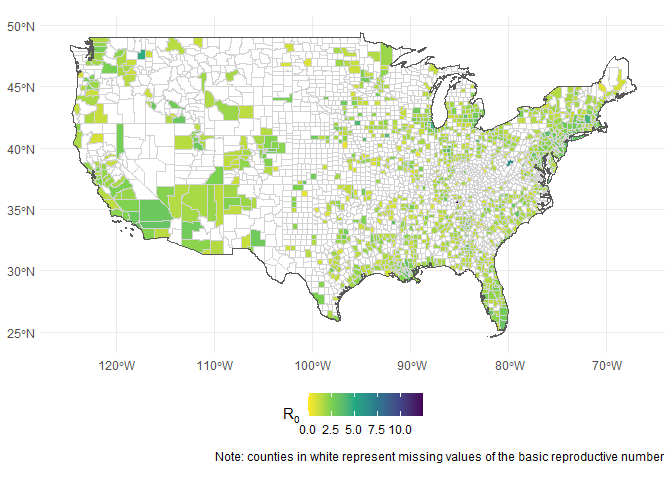
\includegraphics[width=1\linewidth]{R0-Density-Reanalysis_files/figure-latex/R0-map-1} \caption{\label{fig:R0-map}Basic reproductive rate in US counties (Alaska, Hawaii, Puerto Rico, and territories not shown).}\label{fig:R0-map}
\end{figure}

Table \ref{tab:swn-results} reproduces the first three models of SWN
(the fourth model did not have any significant variables; see Table 1 in
SWN). It is possible to verify that the results match, with only the
minor (and irrelevant) exception of the magnitude of the coefficient for
travel by private transportation, which is due to a difference in the
input (here the variable is changed to one percent units, instead of the
ten percent units used by SWN). The mixed linear model gives random
intercepts (i.e., the intercept is a random variable), and the standard
deviation is reported in the \DIFdelbegin \DIFdel{fourth }\DIFdelend \DIFaddbegin \DIFadd{fifth }\DIFaddend row of Table \ref{tab:swn-results}.
It is useful to map the random intercepts: as seen in Figure
\ref{fig:random-terms-map}, other things being equal, counties in Texas
tend to have somewhat lower values of \(R_0\) (i.e., a negative random
intercept), whereas counties in South Dakota tend to have higher values
of \(R_0\). The key of the analysis, after extensive sensitivity
analysis, is a robust finding that population density has a positive
association with the basic reproductive number. But does it?

\begin{table}

\caption{\label{tab:tabulate-swn-results}\label{tab:swn-results}Reproducing SWN: Models 1-3}
\centering
\resizebox{\linewidth}{!}{
\begin{tabular}[t]{lllllrl}
\toprule
\multicolumn{1}{c}{ } & \multicolumn{2}{c}{Model 1} & \multicolumn{2}{c}{Model 2} & \multicolumn{2}{c}{Model 3} \\
\cmidrule(l{3pt}r{3pt}){2-3} \cmidrule(l{3pt}r{3pt}){4-5} \cmidrule(l{3pt}r{3pt}){6-7}
Variable & beta & 95\% CI & beta & 95\% CI & beta & 95\% CI\\
\midrule
Intercept & 2.274 & [2.167, 2.381] & 3.347 & [2.676, 4.018] & 3.386 & [2.614, 4.157]\\
Log of population density & 0.162 & [0.133, 0.191] & 0.145 & [0.115, 0.176] & 0.147 & [0.113, 0.18]\\
Percent of private transportation &  &  & -0.013 & [-0.02, -0.005] & -0.013 & [-0.021, -0.005]\\
Median household income (\$10,000) &  &  &  &  & -0.003 & [-0.033, 0.026]\\
Standard deviation (Intercept) & 0.166 & [0.108, 0.254] & 0.136 & [0.081, 0.229] & 0.137 & [0.081, 0.232]\\
\addlinespace
Within-group standard error & 0.665 & [0.638, 0.693] & 0.665 & [0.638, 0.693] & 0.665 & [0.638, 0.694]\\
\bottomrule
\end{tabular}}
\end{table}

\begin{figure}
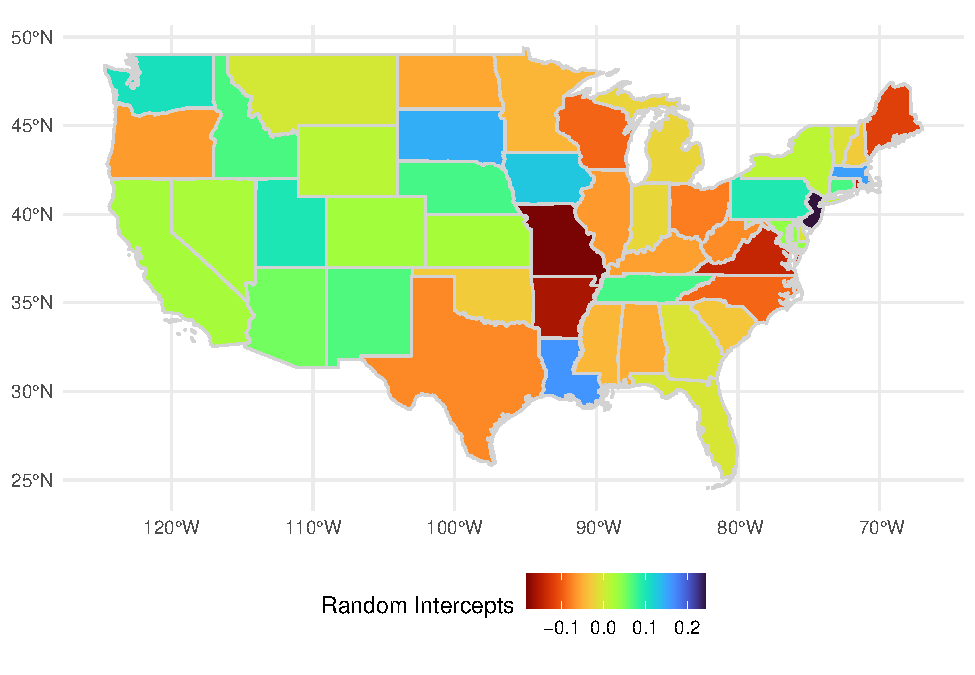
\includegraphics[width=1\linewidth]{R0-Density-Reanalysis_files/figure-latex/random-terms-map-1} \caption{\label{fig:random-terms-map}Random intercepts of Model 3 (Alaska, Hawaii, Puerto Rico, and territories not shown).}\label{fig:random-terms-map}
\end{figure}

\hypertarget{expanding-on-swn}{%
\section{Expanding on SWN}\label{expanding-on-swn}}

The preceding section shows that thanks to the availability of code and
data, it is possible to verify the results reported by SWN. As noted
earlier, though, an independent researcher might have wondered about the
implications of the spatial sampling procedure used by SWN. The decision
to use a sample of counties with reliable basic reproductive numbers,
although apparently sensible, results in a non-random spatial sampling
scheme. Turning our attention back to Figure \ref{fig:R0-map}, we form
the impression that many counties without reliable values of \(R_0\) are
in more rural, less dense parts of the United States. This impression is
reinforced when we overlay the boundaries of urban areas with population
greater than 50,000 on the counties with valid values of \(R_0\) (see
Figure \ref{fig:urban-areas-map}). The fact that \(R_0\) could not be
accurately computed in many counties without large urban areas does not
mean that there was no transmission of the virus: it simply means that
we do not know with sufficient precision to what extent that was the
case. The low number of cases may be related to low population and/or
low population density. This is intriguing, to say the least: by
excluding cases based on the ability to calculate \(R_0\) we are
potentially \emph{selecting} the sample in a non-random way.

\begin{figure}
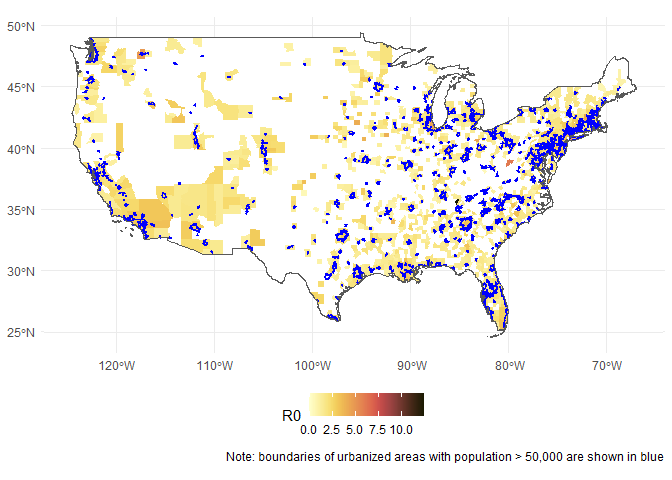
\includegraphics[width=1\linewidth]{R0-Density-Reanalysis_files/figure-latex/urban-areas-map-1} \caption{\label{fig:urban-areas-map}Urban areas with population > 50,000 (Alaska, Hawaii, Puerto Rico, and territories not shown).}\label{fig:urban-areas-map}
\end{figure}

A problematic issue with non-random sample selection is that parameter
estimates can become unreliable, and numerous techniques have been
developed to address this. A model useful for sample selection problems
is Heckman's selection model (see Maddala, 1983). The selection model is
in fact a system of two equations, as follows: \[
\begin{array}{c}
y_i^{S*} = \beta^{S\prime}x_i^S+\epsilon_i^S\\
y_i^{O*} = \beta^{O\prime}x_i^O+\epsilon_i^O
\end{array}
\] \noindent where \(y_i^{S*}\) is a latent variable for the sample
selection process, and \(y_i^{O*}\) is the latent outcome. Vectors
\(x_i^S\) and \(x_i^O\) are explanatory variables (with the possibility
that \(x_i^S = x_i^S\)). Both equations include random terms (i.e.,
\(\epsilon_i^S\) and \(\epsilon_i^O\)). The first equation is designed
to model the \emph{probability} of sampling, and the second equation the
outcome of interest (say \(R_0\)). The random terms are jointly
distributed and correlated with parameter \(\rho\).

What the analyst observes is the following: \[
y_i^S =
\begin{cases}
0 & \text{if } y_i^{S*} < 0\\
1 & \text{otherwise}
\end{cases}
\] \noindent and: \[
y_i^O =
\begin{cases}
0 & \text{if } y_i^{S} = 0\\
y_i^{O*} & \text{otherwise}
\end{cases}
\]

In other words, the outcome of interest is observed \emph{only} for
certain cases (\(y_i^S=1\), i.e., for sampled observations). The
probability of sampling depends on \(x_i^S\). For the cases observed,
the outcome \(y_i^O\) depends on \(x_i^O\).

A sample selection model is estimated using the same selection of
variables as SWN Model 3. This is Sample Selection Model 1 in Table
\ref{tab:selection-results}. The first thing to notice about this model
is that the sample selection process and the outcome are correlated
(\(\rho\ne0\) with 5\% of confidence). The selection equation indicates
that the probability of a county to be in the sample increases with
population density (but at a decreasing rate due to the
log-transformation), when travel by private modes is more prevalent, and
as median household income in the county is higher. This is in line with
the impression made by Figure \ref{fig:urban-areas-map} that counties
with reliable values of \(R_0\) tended to be those with larger urban
centers. Once that the selection probabilities are accounted for in the
model, several things happen with the outcomes model. First, the
coefficient for population density is still positive, but the magnitude
changes: in effect, it appears that the effect of density is more
pronounced than what SWN Model 3 indicated. The coefficient for percent
of private transportation changes signs. And the coefficient for median
household income is now significant.

The second model in Table \ref{tab:selection-results} (Selection Model
2) changes the way the variables are entered into the model. The
log-transformation of density in SWN and Selection Model 1 assumes that
the association between density and \(R_0\) is monotonically increasing
(if the sign of the coefficient is positive) or decreasing (if the sign
of the coefficient is negative). There are some indications that the
relationship may actually not be monotonical. For example, Paez et al.
(2020) found a positive (if non-significant) relationship between
density and incidence of COVID-19 in the provinces of Spain at the
beginning of the pandemic. This changed to a negative (and significant)
relationship during the lockdown. In the case of the US, Fielding-Miller
et al. (2020) found that the association between COVID-19 deaths and
population density was positive in rural counties, but negative in urban
counties. A variable transformation that allows for non-monotonic
changes in the relationship is the square of the density.

As seen in the table, Selection Model 2 replaces the log-transformation
of population density with a quadratic expansion. The results of this
analysis indicate that with this variable transformation, the selection
and outcome processes are still correlated (\(\rho\ne0\) with 5\% of
confidence). But a few other interesting things emerge. When we examine
the outcomes model, we see that the quadratic expansion has a positive
coefficient for the first order term, but a negative coefficient for the
second order term. This indicates that \(R_0\) initially tends to
increase as density grows, but only up to a point, after which the
negative second term (which grows more rapidly due to the square),
becomes increasingly dominant. Secondly, the sign of the coefficient for
travel by private transportation becomes negative again. This, of
course, makes more sense than the positive sign of Selection Model 1: if
people tend to travel in private transportation, the potential for
contact should be lower instead of higher. And finally median household
income is no longer significant, similar to SWN Model 3.

\begin{table}

\caption{\label{tab:tabulate-sample-selection-results}\label{tab:selection-results}Estimation results of sample selection models}
\centering
\resizebox{\linewidth}{!}{
\begin{tabular}[t]{lcccc}
\toprule
\multicolumn{1}{c}{ } & \multicolumn{2}{c}{Selection Model 1} & \multicolumn{2}{c}{Selection Model 2} \\
\cmidrule(l{3pt}r{3pt}){2-3} \cmidrule(l{3pt}r{3pt}){4-5}
Variable & $\beta$ & 95\% CI & $\beta$ & 95\% CI\\
\midrule
\addlinespace[0.3em]
\multicolumn{5}{l}{\textbf{Sample Selection Model}}\\
\hspace{1em}Intercept & -2.237 & [-3.109, -1.365] & -7.339 & [-8.381, -6.297]\\
\hspace{1em}Log of population density & 0.385 & [0.352, 0.418] &  & \\
\hspace{1em}Density (1,000 per sq.km) &  &  & 2.484 & [2.13, 2.838]\\
\hspace{1em}Density squared &  &  & -0.387 & [-0.473, -0.3]\\
\hspace{1em}Percent of private transportation & 0.025 & [0.016, 0.034] & 0.057 & [0.046, 0.067]\\
\hspace{1em}Median household income (10,000) & 0.202 & [0.168, 0.235] & 0.32 & [0.283, 0.357]\\
\addlinespace[0.3em]
\multicolumn{5}{l}{\textbf{Outcome Model}}\\
\hspace{1em}Intercept & 0.605 & [-0.257, 1.466] & 2.784 & [1.652, 3.915]\\
\hspace{1em}Log of population density & 0.39 & [0.354, 0.426] &  & \\
\hspace{1em}Density (1,000 per sq.km) &  &  & 0.758 & [0.509, 1.008]\\
\hspace{1em}Density squared &  &  & -0.132 & [-0.187, -0.077]\\
\hspace{1em}Percent of private transportation & 0.01 & [0.001, 0.018] & -0.011 & [-0.021, -0.001]\\
\hspace{1em}Median household income (\$10,000) & 0.126 & [0.094, 0.159] & 0.002 & [-0.033, 0.037]\\
$\sigma$ & 0.954 & [0.904, 1.003] & 0.684 & [0.652, 0.716]\\
$\rho$ & 0.971 & [0.961, 0.98] & -0.199 & [-0.377, -0.022]\\
\bottomrule
\end{tabular}}
\end{table}

\hypertarget{proceed-with-caution-spatial-effects-ahead}{%
\section{Proceed with caution: spatial effects
ahead}\label{proceed-with-caution-spatial-effects-ahead}}

The results of the selection models, in particular Selection Model 2,
make us reassess the original conclusion that density has a positive
association with the basic reproductive number of COVID-19. A spatial
analyst might still wonder about spatial residual autocorrelation. A
challenge here is that spatial models tend to be technically more
demanding, and although spatial models for qualitative variables exist,
a spatial implementation of the sample selection model does not appear
to exist. It might be argued that a reproducible research project can
also allow a researcher to be more adventurous with their modeling
decisions: since data and code are shared, other researchers can
promptly and with relative ease poke the methods and see if they appear
to be sound.

In the present case, it appears that an application of spatial filtering
(see Getis and Griffith, 2002; Griffith, 2004; Paez, 2019) can help.
Spatial filtering provides an elegant solution to regression problems
that may have difficulties handling the spatial structures of spatial
statistical and econometric models (Griffith, 2000). A key issue in the
present example is the fact that there are numerous missing
observations, which prevents the calculation of autocorrelation
statistics, let alone the estimation of models with spatial components.

The following is an unorthodox, but potentially effective use of filters
in a sample selection model:

\begin{enumerate}
\def\labelenumi{\arabic{enumi}.}
\item
  Estimate a sample selection model and retrieve the residuals of the
  outcome. This will be a vector with missing values for locations that
  were not sampled.
\item
  Fit a spatial filter to the residuals. This is done by regressing the
  estimated residuals of the \emph{observed} data on the corresponding
  values of the Moran eigenvectors.
\item
  The resulting filter will correlate highly with the known residuals,
  and will provide information in non-sampled locations that is
  consistent with the spatial pattern of the known residuals.
\item
  Test the filter for spatial autocorrelation:

  4.1 If significant spatial autocorrelation is detected, this would be
  indicative of residual spatial pattern. Introduce the filter as a
  covariate in the outcome model of the sample selection model and
  return to step 1.

  4.2 If no significant spatial autocorrelation is detected, this would
  be indicative of random residual pattern. Stop.
\end{enumerate}

This procedure is implemented using a stopping criterion whereby the
search for the filter only stops when the p-value of Moran's Coefficient
of the filter fitted to the residuals is greater than 0.25, which was
chosen as a sufficiently conservative value for testing for
autocorrelation. The correlation of the known residuals with the
corresponding elements of the filter is consistently high (the
correlation coefficient typically is greater than 0.9). The results of
implementing this procedure appear in Table \ref{tab:selection3-results}
as Selection Model 3. The results are consistent with Selection Model 2,
with two intriguing differences: 1) the variance of Sample Model 3 is
smaller; and 2) the sample and outcome processes are no longer
correlated (the confidence interval of \(\rho\) includes zero). It
appears that by capturing the spatial pattern of the residuals, which is
likely strongly determined by the non-random sampling framework, the
outcome model is not only substantially more precise, but also appears
to be independent from the selection process.

\begin{table}[!h]

\caption{\label{tab:tabulate-sample-selection3-results}\label{tab:selection3-results}Estimation results of sample selection model with spatial filter}
\centering
\fontsize{8}{10}\selectfont
\begin{tabular}[t]{lcc}
\toprule
\multicolumn{1}{c}{ } & \multicolumn{2}{c}{Selection Model 3} \\
\cmidrule(l{3pt}r{3pt}){2-3}
Variable & $\beta$ & 95\% CI\\
\midrule
\addlinespace[0.3em]
\multicolumn{3}{l}{\textbf{Sample Selection Model}}\\
\hspace{1em}Intercept & -7.304 & [-8.346, -6.262]\\
\hspace{1em}Density (1,000 per sq.km) & 2.445 & [2.089, 2.802]\\
\hspace{1em}Density squared & -0.380 & [-0.468, -0.292]\\
\hspace{1em}Percent of private transportation & 0.056 & [0.046, 0.067]\\
\hspace{1em}Median household income (10,000) & 0.318 & [0.28, 0.356]\\
\addlinespace[0.3em]
\multicolumn{3}{l}{\textbf{Outcome Model}}\\
\hspace{1em}Intercept & 2.563 & [2.497, 2.629]\\
\hspace{1em}Density (1,000 per sq.km) & 0.760 & [0.746, 0.774]\\
\hspace{1em}Density squared & -0.133 & [-0.135, -0.13]\\
\hspace{1em}Percent of private transportation & -0.011 & [-0.012, -0.011]\\
\hspace{1em}Median household income (\$10,000) & 0.002 & [-0.001, 0.004]\\
\hspace{1em}Spatial filter & 1.000 & [0.998, 1.001]\\
$\sigma$ & 0.017 & [0.015, 0.019]\\
$\rho$ & -0.304 & [-0.957, 0.349]\\
\bottomrule
\end{tabular}
\end{table}

\DIFdelbegin %DIFDELCMD < \hypertarget{discussion}{%
%DIFDELCMD < \section{Discussion}\label{discussion}}
%DIFDELCMD < 

%DIFDELCMD < %%%
\DIFdel{How relevant are the differences between the various model
specifications presented above}\DIFdelend \DIFaddbegin \DIFadd{Clearly, the various models display some intriguing differences; but how
relevant are said differences from a more substantive standpoint}\DIFaddend ? Figure
\ref{fig:comparison-results} shows the relationship between density and
\(R_0\) implied by SWN Model 3, Selection Model 2, and Selection Model
3. The left panel of the figure shows the non-linear but monotonic
relationship implied by SWN Model 1. The conclusion is that at higher
densities, \(R_0\) is \emph{always} higher. The two panels on the right,
in contrast, shows that Selection Model 2 and Selection Model 3 coincide
that \(R_0\) tends to increase as density grows. This continues until a
density of approximately 2.9 (1,000 people per sq.km). At higher
densities than that the relationship between density and \(R_0\) begins
to weaken, and the relationship becomes negative at densities higher
than approximately 5.7 (1,000 people per sq.km).

To put this into context, other things being equal, the effect of
density in a county like Charlottesville in Virginia (density
\textasciitilde1,639 people per sq.km) is roughly the same as that in a
county like Philadelphia (density \textasciitilde4,127 people per
sq.km). In contrast, the effect of density on \(R_0\) in a county like
Arlington in Virginia (density \textasciitilde3,093 people per sq.km) is
\emph{stronger} than either of the previous two examples. Lastly, the
density of counties like San Francisco in California, or Queens and
Bronx in NY, which are among the densest in the US, contributes even
less to \(R_0\) than even the most rural counties in the country.

\DIFaddbegin \begin{figure}
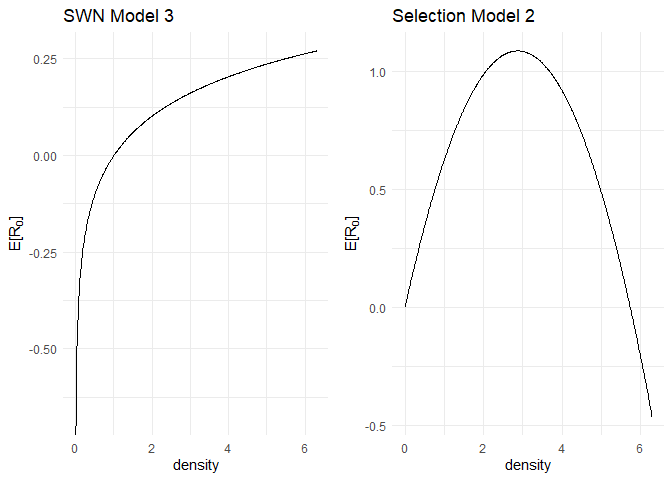
\includegraphics[width=1\linewidth]{R0-Density-Reanalysis_files/figure-latex/comparison-results-1} \caption{\label{fig:comparison-results}\DIFaddFL{Effect of density according to SWN Model 3 and Sample Selection Model 2.}}\label{fig:comparison-results}
\end{figure}

\hypertarget{discussion}{%
\section{Discussion}\label{discussion}}

\DIFaddend It is worth at this point to recall Cressie's dictum about modelling:
``{[}w{]}hat is one person's mean structure could be another person's
correlation structure'' (Cressie, 1989, p. 201). There are almost always
multiple ways to approach a modelling situation\DIFdelbegin \DIFdel{. }\DIFdelend \DIFaddbegin \DIFadd{, as lively illustrated
by a recent paper that reports the results of a crowdsourced modelling
experiment (Schweinsberg et al., 2021). }\DIFaddend In the present case, we would
argue that spatial sampling is an important aspect of the modeling
process\DIFdelbegin \DIFdel{, but one that perhaps required different technical skills than
those available to SWN. There is nothing wrong with that. What matters
is that}\DIFdelend \DIFaddbegin \DIFadd{. Importantly}\DIFaddend , by adopting \DIFdelbegin \DIFdel{relatively }\DIFdelend high reproducibility standards, \DIFdelbegin \DIFdel{these
researchers }\DIFdelend \DIFaddbegin \DIFadd{SWN
}\DIFaddend made a valuable \DIFdelbegin \DIFdel{and honest }\DIFdelend contribution to the collective enterprise of seeking
knowledge. Their effort, and subsequent efforts to validate and expand
on their work, can potentially contribute to provide clarity to ongoing
conversations about the relevance of density and the spread of COVID-19.

In particular, it is noteworthy that a sample selection model with a
different variable transformation does not lend support to the thesis
that higher density is \emph{always} associated with a greater risk of
spread of the virus {[}\DIFdelbegin \DIFdel{as put by }\DIFdelend \DIFaddbegin \DIFadd{in }\DIFaddend Wong and Li\DIFaddbegin \DIFadd{'s words}\DIFaddend , ``\,`Density is destiny'
is probably an overstatement''; (2020){]}. At the same time, \DIFdelbegin \DIFdel{this also stands }\DIFdelend \DIFaddbegin \DIFadd{the results
presented here also stand }\DIFaddend in contrast to the findings of Hamidi et al.,
who found that higher density was either not significantly associated
with the rate of the virus in a cross-sectional study (Hamidi et al.,
2020b), or was negatively associated with it in a longitudinal setting
{[}Hamidi et al. (2020a). In this sense, the conclusion that density
does not aggravate the pandemic may have been somewhat premature;
instead, reanalysis of the data of SWN suggests that Fielding-Miller et
al. (2020) might be onto something with respect to the difference
between rural and urban counties. More generally, there is no doubt that
in population-level studies density is indicative of proximity, but it
also potentially is a proxy for adaptive behavior. And it is possible
that the determining factor during COVID-19, at least in the US, has
been variations in perceptions of the risks associated with contagion
(Chauhan et al., 2021), and subsequent compensations in behavior in more
and less dense regions.

\DIFdelbegin %DIFDELCMD < \begin{figure}
%DIFDELCMD < 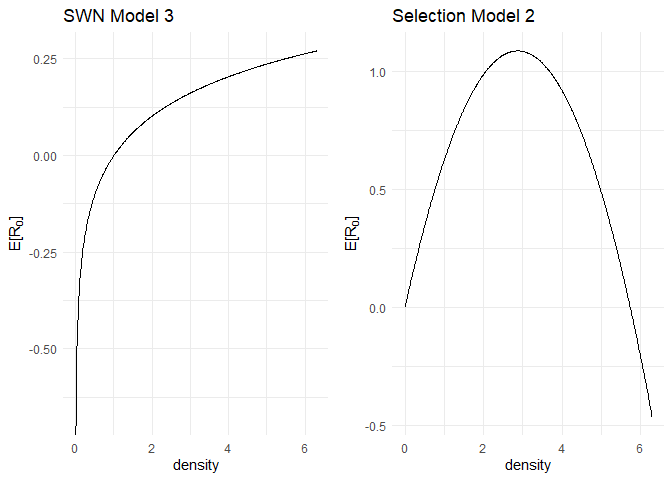
\includegraphics[width=1\linewidth]{R0-Density-Reanalysis_files/figure-latex/comparison-results-1} %%%
%DIFDELCMD < \caption{%
{%DIFAUXCMD
%DIFDELCMD < \label{fig:comparison-results}%%%
\DIFdelFL{Effect of density according to SWN Model 3 and Sample Selection Model 2.}}%DIFAUXCMD
%DIFDELCMD < \label{fig:comparison-results}
%DIFDELCMD < \end{figure}
%DIFDELCMD < 

%DIFDELCMD < %%%
\DIFdelend \hypertarget{conclusion}{%
\section{Conclusion}\label{conclusion}}

The tension between the need to publish research potentially useful in
dealing with a global pandemic, and a potential ``carnage of substandard
research'' (Bramstedt, 2020), highlights the importance of efforts to
maintain the quality of scientific outputs during COVID-19. An important
part of quality control is the ability of independent researchers to
verify and examine the results of materials published in the literature.
As previous research illustrates, reproducibility in scientific research
remains an important but elusive goal (Gustot, 2020; e.g., Iqbal et al.,
2016; Stodden et al., 2018; Sumner et al., 2020). This idea is
reinforced by the review conducted for this paper in the context of
research about population density and the spread of COVID-19.

Taking one recent example from the literature {[}Sy et al., Sy et al.
(2021); SWN{]}, the present paper illustrates the importance of good
reproducibility practices. Sharing data and code can catalyze research,
by allowing independent verification of findings, as well as additional
research. After verifying the results of SWN, experiments with sample
selection models and variations in the definition of model inputs, lead
to an important reappraisal of the conclusion that high density is
associated with greater spread of the virus. Instead, the possibility of
a non-monotonical relationship between population density and contagion
is raised. \DIFaddbegin \DIFadd{I do not claim that the analysis presented here is the last
word on the topic of density and the spread of COVID-19, and there is
always the possibility that someone else will be better equipped to
analyze these data with greater competence. By opening up the analysis,
documenting the way data were pre-processed, and by sharing analysis
ready data, my hope would be that others will be able to discover the
limitations of my own analysis and improve on it, as appropriate.
}\DIFaddend 

\DIFdelbegin \DIFdel{In the spirit of openness, this paper is
prepared as an R Markdown
document, an a companion data package is provided. The data package
contains the relevant documentation of the data, }\DIFdelend \DIFaddbegin \DIFadd{More generally, my hope is that the research of Sy et al. (2021), the
present paper, }\DIFaddend and \DIFdelbegin \DIFdel{all datapre-processing is fully documented. Hopefully this, and }\DIFdelend similar reproducible \DIFdelbegin \DIFdel{papers}\DIFdelend \DIFaddbegin \DIFadd{publications}\DIFaddend , will continue to
encourage others to adopt \DIFdelbegin \DIFdel{reproducible }\DIFdelend \DIFaddbegin \DIFadd{higher reproducibility }\DIFaddend standards in their
research.

\hypertarget{references}{%
\section*{References}\label{references}}
\addcontentsline{toc}{section}{References}

\hypertarget{refs}{}
\begin{CSLReferences}{1}{0}
\leavevmode\hypertarget{ref-Ahmad2020association}{}%
Ahmad, K., Erqou, S., Shah, N., Nazir, U., Morrison, A.R., Choudhary,
G., Wu, W.-C., 2020. Association of poor housing conditions with
COVID-19 incidence and mortality across US counties. PLOS ONE 15,
e0241327.
doi:\href{https://doi.org/10.1371/journal.pone.0241327}{10.1371/journal.pone.0241327}

\leavevmode\hypertarget{ref-Amadu2021assessing}{}%
Amadu, I., Ahinkorah, B.O., Afitiri, A.-R., Seidu, A.-A., Ameyaw, E.K.,
Hagan, J.E., Duku, E., Aram, S.A., 2021. Assessing sub-regional-specific
strengths of healthcare systems associated with COVID-19 prevalence,
deaths and recoveries in africa. PLOS ONE 16, e0247274.
doi:\href{https://doi.org/10.1371/journal.pone.0247274}{10.1371/journal.pone.0247274}

\leavevmode\hypertarget{ref-Anazco2021publication}{}%
Añazco, D., Nicolalde, B., Espinosa, I., Camacho, J., Mushtaq, M.,
Gimenez, J., Teran, E., 2021. Publication rate and citation counts for
preprints released during the COVID-19 pandemic: The good, the bad and
the ugly. PeerJ 9, e10927.
doi:\href{https://doi.org/10.7717/peerj.10927}{10.7717/peerj.10927}

\leavevmode\DIFaddbegin \hypertarget{ref-Arribas2021open}{}%DIF > 
\DIFadd{Arribas-Bel, D., Green, M., Rowe, F., Singleton, A., 2021. Open data
products: A framework for creating valuable analysis-ready data. Journal
of Geographical Systems.
}

\leavevmode\DIFaddend \hypertarget{ref-Basu2017ten}{}%
Basu, S., Carney, M.A., Kenworthy, N.J., 2017. Ten years after the
financial crisis: The long reach of austerity and its global impacts on
health. Social Science \& Medicine 187, 203--207.
doi:\href{https://doi.org/10.1016/j.socscimed.2017.06.026}{10.1016/j.socscimed.2017.06.026}

\leavevmode\hypertarget{ref-Bhadra2021impact}{}%
Bhadra, A., Mukherjee, A., Sarkar, K., 2021. Impact of population
density on covid-19 infected and mortality rate in india. Modeling Earth
Systems and Environment 7, 623--629.
doi:\href{https://doi.org/10.1007/s40808-020-00984-7}{10.1007/s40808-020-00984-7}

\leavevmode\DIFaddbegin \hypertarget{ref-Bivand2020progress}{}%DIF > 
\DIFadd{Bivand, R.S., 2020. Progress in the r ecosystem for representing and
handling spatial data. Journal of Geographical Systems.
doi:}\href{https://doi.org/10.1007/s10109-020-00336-0}{\DIFadd{10.1007/s10109-020-00336-0}}

\leavevmode\DIFaddend \hypertarget{ref-Bramstedt2020carnage}{}%
Bramstedt, K.A., 2020. The carnage of substandard research during the
COVID-19 pandemic: A call for quality. Journal of Medical Ethics 46,
803--807.
doi:\href{https://doi.org/10.1136/medethics-2020-106494}{10.1136/medethics-2020-106494}

\leavevmode\hypertarget{ref-Brandtner2021creatures}{}%
Brandtner, C., Bettencourt, L.M.A., Berman, M.G., Stier, A.J., 2021.
Creatures of the state? Metropolitan counties compensated for state
inaction in initial u.s. Response to COVID-19 pandemic. PLOS ONE 16,
e0246249.
doi:\href{https://doi.org/10.1371/journal.pone.0246249}{10.1371/journal.pone.0246249}

\leavevmode\hypertarget{ref-Broggini2017reproducible}{}%
Broggini, F., Dellinger, J., Fomel, S., Liu, Y., 2017. Reproducible
research: Geophysics papers of the future - introduction. Geophysics 82.
doi:\href{https://doi.org/10.1190/geo2017-0918-spseintro.1}{10.1190/geo2017-0918-spseintro.1}

\leavevmode\hypertarget{ref-Brunsdon2020opening}{}%
Brunsdon, C., Comber, A., 2020. Opening practice: Supporting
reproducibility and critical spatial data science. Journal of
Geographical Systems.
doi:\href{https://doi.org/10.1007/s10109-020-00334-2}{10.1007/s10109-020-00334-2}

\leavevmode\hypertarget{ref-Chauhan2021covid}{}%
Chauhan, R.S., Capasso da Silva, D., Salon, D., Shamshiripour, A.,
Rahimi, E., Sutradhar, U., Khoeini, S., Mohammadian, A.(Kouros).,
Derrible, S., Pendyala, R., 2021. COVID-19 related attitudes and risk
perceptions across urban, rural, and suburban areas in the united
states. Findings.
doi:\href{https://doi.org/10.32866/001c.23714}{10.32866/001c.23714}

\leavevmode\hypertarget{ref-Cressie1989geostatistics}{}%
Cressie, N., 1989. Geostatistics. The American Statistician 43, 197.
doi:\href{https://doi.org/10.2307/2685361}{10.2307/2685361}

\leavevmode\hypertarget{ref-Cruz2020exploring}{}%
Cruz, C.J.P., Ganly, R., Li, Z., Gietel-Basten, S., 2020. Exploring the
young demographic profile of COVID-19 cases in hong kong: Evidence from
migration and travel history data. PLOS ONE 15, e0235306.
doi:\href{https://doi.org/10.1371/journal.pone.0235306}{10.1371/journal.pone.0235306}

\leavevmode\hypertarget{ref-Farber2011running}{}%
Farber, S., Páez, A., 2011. Running to stay in place: The time-use
implications of automobile oriented land-use and travel. Journal of
Transport Geography 19, 782--793.
doi:\href{https://doi.org/10.1016/j.jtrangeo.2010.09.008}{10.1016/j.jtrangeo.2010.09.008}

\leavevmode\hypertarget{ref-Feng2020spread}{}%
Feng, Y., Li, Q., Tong, X., Wang, R., Zhai, S., Gao, C., Lei, Z., Chen,
S., Zhou, Y., Wang, J., Yan, X., Xie, H., Chen, P., Liu, S., Xv, X.,
Liu, S., Jin, Y., Wang, C., Hong, Z., Luan, K., Wei, C., Xu, J., Jiang,
H., Xiao, C., Guo, Y., 2020. Spatiotemporal spread pattern of the
COVID-19 cases in china. PLOS ONE 15, e0244351.
doi:\href{https://doi.org/10.1371/journal.pone.0244351}{10.1371/journal.pone.0244351}

\leavevmode\hypertarget{ref-Feyman2020effectiveness}{}%
Feyman, Y., Bor, J., Raifman, J., Griffith, K.N., 2020. Effectiveness of
COVID-19 shelter-in-place orders varied by state. PLOS ONE 15, e0245008.
doi:\href{https://doi.org/10.1371/journal.pone.0245008}{10.1371/journal.pone.0245008}

\leavevmode\hypertarget{ref-Fielding2020social}{}%
Fielding-Miller, R.K., Sundaram, M.E., Brouwer, K., 2020. Social
determinants of COVID-19 mortality at the county level. PLOS ONE 15,
e0240151.
doi:\href{https://doi.org/10.1371/journal.pone.0240151}{10.1371/journal.pone.0240151}

\leavevmode\hypertarget{ref-Florida2020how}{}%
Florida, R., Glaeser, E., Sharif, M., Bedi, K., Campanella, T., Chee,
C., Doctoroff, D., Katz, B., Katz, R., Kotkin, J., 2020. How life in our
cities will look after the coronavirus pandemic. Foreign Policy 1.

\leavevmode\hypertarget{ref-Fraser2021evolving}{}%
Fraser, N., Brierley, L., Dey, G., Polka, J.K., Pálfy, M., Nanni, F.,
Coates, J.A., 2021. The evolving role of preprints in the dissemination
of COVID-19 research and their impact on the science communication
landscape. PLOS Biology 19, e3000959.
doi:\href{https://doi.org/10.1371/journal.pbio.3000959}{10.1371/journal.pbio.3000959}

\leavevmode\hypertarget{ref-Getis2002comparative}{}%
Getis, A., Griffith, D.A., 2002. Comparative spatial filtering in
regression analysis. Geographical Analysis 34, 130--140.

\leavevmode\hypertarget{ref-Gomez2021infekta}{}%
Gomez, J., Prieto, J., Leon, E., Rodríguez, A., 2021. INFEKTA---an
agent-based model for transmission of infectious diseases: The COVID-19
case in bogotá, colombia. PLOS ONE 16, e0245787.
doi:\href{https://doi.org/10.1371/journal.pone.0245787}{10.1371/journal.pone.0245787}

\leavevmode\hypertarget{ref-Griffith2000linear}{}%
Griffith, D.A., 2000. A linear regression solution to the spatial
autocorrelation problem. Journal of Geographical Systems 2, 141--156.

\leavevmode\hypertarget{ref-Griffith2004spatial}{}%
Griffith, D.A., 2004. A spatial filtering specification for the
autologistic model. Environment and Planning A 36, 1791--1811.

\leavevmode\hypertarget{ref-Gustot2020quality}{}%
Gustot, T., 2020. Quality and reproducibility during the COVID-19
pandemic. JHEP Rep 2, 100141.
doi:\href{https://doi.org/10.1016/j.jhepr.2020.100141}{10.1016/j.jhepr.2020.100141}

\leavevmode\hypertarget{ref-Hamidi2020longitudinal}{}%
Hamidi, S., Ewing, R., Sabouri, S., 2020a. Longitudinal analyses of the
relationship between development density and the COVID-19 morbidity and
mortality rates: Early evidence from 1,165 metropolitan counties in the
united states. Health \& Place 64, 102378.
doi:\href{https://doi.org/10.1016/j.healthplace.2020.102378}{10.1016/j.healthplace.2020.102378}

\leavevmode\hypertarget{ref-Hamidi2020density}{}%
Hamidi, S., Sabouri, S., Ewing, R., 2020b. Does density aggravate the
COVID-19 pandemic? Journal of the American Planning Association 86,
495--509.
doi:\href{https://doi.org/10.1080/01944363.2020.1777891}{10.1080/01944363.2020.1777891}

\leavevmode\hypertarget{ref-Hamidi2021compact}{}%
Hamidi, S., Zandiatashbar, A., 2021. Compact development and adherence
to stay-at-home order during the COVID-19 pandemic: A longitudinal
investigation in the united states. Landscape and Urban Planning 205,
103952. doi:\url{https://doi.org/10.1016/j.landurbplan.2020.103952}

\leavevmode\hypertarget{ref-Harris2021Changes}{}%
Harris, M.A., Branion-Calles, M., 2021. Changes in commute mode
attributed to COVID-19 risk in canadian national survey data. Findings.
doi:\href{https://doi.org/10.32866/001c.19088}{10.32866/001c.19088}

\leavevmode\hypertarget{ref-Herndon2014high}{}%
Herndon, T., Ash, M., Pollin, R., 2014. Does high public debt
consistently stifle economic growth? A critique of reinhart and rogoff.
Cambridge Journal of Economics 38, 257--279.
doi:\href{https://doi.org/10.1093/cje/bet075}{10.1093/cje/bet075}

\leavevmode\hypertarget{ref-Inbaraj2021seroprevalence}{}%
Inbaraj, L.R., George, C.E., Chandrasingh, S., 2021. Seroprevalence of
COVID-19 infection in a rural district of south india: A
population-based seroepidemiological study. PLOS ONE 16, e0249247.
doi:\href{https://doi.org/10.1371/journal.pone.0249247}{10.1371/journal.pone.0249247}

\leavevmode\hypertarget{ref-Ince2012case}{}%
Ince, D.C., Hatton, L., Graham-Cumming, J., 2012. The case for open
computer programs. Nature 482, 485--488.
doi:\href{https://doi.org/10.1038/nature10836}{10.1038/nature10836}

\leavevmode\hypertarget{ref-Ioannidis2014increasing}{}%
Ioannidis, J.P.A., Greenland, S., Hlatky, M.A., Khoury, M.J., Macleod,
M.R., Moher, D., Schulz, K.F., Tibshirani, R., 2014. Increasing value
and reducing waste in research design, conduct, and analysis. Lancet
383, 166--175.
doi:\href{https://doi.org/10.1016/s0140-6736(13)62227-8}{10.1016/s0140-6736(13)62227-8}

\leavevmode\hypertarget{ref-Iqbal2016reproducible}{}%
Iqbal, S.A., Wallach, J.D., Khoury, M.J., Schully, S.D., Ioannidis,
J.P.A., 2016. Reproducible research practices and transparency across
the biomedical literature. Plos Biology 14.
doi:\href{https://doi.org/10.1371/journal.pbio.1002333}{10.1371/journal.pbio.1002333}

\leavevmode\hypertarget{ref-Jamal2020Changes}{}%
Jamal, S., Paez, A., 2020. Changes in trip-making frequency by mode
during COVID-19. Findings.
doi:\href{https://doi.org/10.32866/001c.17977}{10.32866/001c.17977}

\leavevmode\hypertarget{ref-Kadi2020population}{}%
Kadi, N., Khelfaoui, M., 2020. Population density, a factor in the
spread of COVID-19 in algeria: Statistic study. Bulletin of the National
Research Centre 44.
doi:\href{https://doi.org/10.1186/s42269-020-00393-x}{10.1186/s42269-020-00393-x}

\leavevmode\hypertarget{ref-Khavarian2021high}{}%
Khavarian-Garmsir, A.R., Sharifi, A., Moradpour, N., 2021. Are
high-density districts more vulnerable to the COVID-19 pandemic?
Sustainable Cities and Society 70, 102911.
doi:\href{https://doi.org/10.1016/j.scs.2021.102911}{10.1016/j.scs.2021.102911}

\leavevmode\hypertarget{ref-Konkol2019examination}{}%
Konkol, M., Kray, C., 2019. In-depth examination of spatiotemporal
figures in open reproducible research. Cartography and Geographic
Information Science 46, 412--427.
doi:\href{https://doi.org/10.1080/15230406.2018.1512421}{10.1080/15230406.2018.1512421}

\leavevmode\hypertarget{ref-Konkol2019computational}{}%
Konkol, M., Kray, C., Pfeiffer, M., 2019. Computational reproducibility
in geoscientific papers: Insights from a series of studies with
geoscientists and a reproduction study. International Journal of
Geographical Information Science 33, 408--429.
doi:\href{https://doi.org/10.1080/13658816.2018.1508687}{10.1080/13658816.2018.1508687}

\leavevmode\hypertarget{ref-Kwon2021swamped}{}%
Kwon, D., 2020. How swamped preprint servers are blocking bad
coronavirus research. Nature 581, 130--132.

\leavevmode\hypertarget{ref-Lee2020human}{}%
Lee, M., Zhao, J., Sun, Q., Pan, Y., Zhou, W., Xiong, C., Zhang, L.,
2020. Human mobility trends during the early stage of the COVID-19
pandemic in the united states. PLOS ONE 15, e0241468.
doi:\href{https://doi.org/10.1371/journal.pone.0241468}{10.1371/journal.pone.0241468}

\leavevmode\hypertarget{ref-Li2018effect}{}%
Li, R., Richmond, P., Roehner, B.M., 2018. Effect of population density
on epidemics. Physica A: Statistical Mechanics and its Applications 510,
713--724.
doi:\href{https://doi.org/10.1016/j.physa.2018.07.025}{10.1016/j.physa.2018.07.025}

\leavevmode\hypertarget{ref-Maddala1983limited}{}%
Maddala, G.S., 1983. Limited-dependent and qualitative variables in
econometrics. Cambridge University Press, Cambridge.

\leavevmode\hypertarget{ref-Micallef2020first}{}%
Micallef, S., Piscopo, T.V., Casha, R., Borg, D., Vella, C., Zammit,
M.-A., Borg, J., Mallia, D., Farrugia, J., Vella, S.M., Xerri, T.,
Portelli, A., Fenech, M., Fsadni, C., Mallia Azzopardi, C., 2020. The
first wave of COVID-19 in malta; a national cross-sectional study. PLOS
ONE 15, e0239389.
doi:\href{https://doi.org/10.1371/journal.pone.0239389}{10.1371/journal.pone.0239389}

\leavevmode\hypertarget{ref-Molloy2020Tracing}{}%
Molloy, J., Tchervenkov, C., Hintermann, B., Axhausen, K.W., 2020.
Tracing the sars-CoV-2 impact: The first month in switzerland. Findings.
doi:\href{https://doi.org/10.32866/001c.12903}{10.32866/001c.12903}

\leavevmode\hypertarget{ref-Moore1970some}{}%
Moore, E.G., 1970. Some spatial properties of urban contact fields.
Geographical Analysis 2, 376--386.

\leavevmode\hypertarget{ref-Moore1970urban}{}%
Moore, E.G., Brown, L.A., 1970. Urban acquaintance fields: An evaluation
of a spatial model. Environment and Planning 2, 443--454.

\leavevmode\hypertarget{ref-Noland1995perceived}{}%
Noland, R.B., 1995. PERCEIVED RISK AND MODAL CHOICE - RISK COMPENSATION
IN TRANSPORTATION SYSTEM. Accident Analysis and Prevention 27, 503--521.
doi:\href{https://doi.org/10.1016/0001-4575(94)00087-3}{10.1016/0001-4575(94)00087-3}

\leavevmode\hypertarget{ref-Noland2021mobility}{}%
Noland, R.B., 2021. Mobility and the effective reproduction rate of
COVID-19. Journal of Transport \& Health 20, 101016.
doi:\url{https://doi.org/10.1016/j.jth.2021.101016}

\leavevmode\hypertarget{ref-Noury2021how}{}%
Noury, A., François, A., Gergaud, O., Garel, A., 2021. How does COVID-19
affect electoral participation? Evidence from the french municipal
elections. PLOS ONE 16, e0247026.
doi:\href{https://doi.org/10.1371/journal.pone.0247026}{10.1371/journal.pone.0247026}

\leavevmode\hypertarget{ref-Paez2019using}{}%
Paez, A., 2019. Using spatial filters and exploratory data analysis to
enhance regression models of spatial data. Geographical Analysis 51,
314--338.
doi:\href{https://doi.org/10.1111/gean.12180}{10.1111/gean.12180}

\leavevmode\hypertarget{ref-Paez2020using}{}%
Paez, A., 2020. Using google community mobility reports to investigate
the incidence of COVID-19 in the united states. Findings.
doi:\url{https://doi.org/10.32866/001c.12976}

\leavevmode\hypertarget{ref-Paez2020spatio}{}%
Paez, A., Lopez, F.A., Menezes, T., Cavalcanti, R., Pitta, M.G. da R.,
2020. A spatio-temporal analysis of the environmental correlates of
COVID-19 incidence in spain. Geographical Analysis n/a.
doi:\href{https://doi.org/10.1111/gean.12241}{10.1111/gean.12241}

\leavevmode\hypertarget{ref-Pequeno2020air}{}%
Pequeno, P., Mendel, B., Rosa, C., Bosholn, M., Souza, J.L., Baccaro,
F., Barbosa, R., Magnusson, W., 2020. Air transportation, population
density and temperature predict the spread of COVID-19 in brazil. PeerJ
8, e9322.
doi:\href{https://doi.org/10.7717/peerj.9322}{10.7717/peerj.9322}

\leavevmode\hypertarget{ref-Phillips2011risk}{}%
Phillips, R.O., Fyhri, A., Sagberg, F., 2011. Risk compensation and
bicycle helmets. Risk Analysis 31, 1187--1195.
doi:\href{https://doi.org/10.1111/j.1539-6924.2011.01589.x}{10.1111/j.1539-6924.2011.01589.x}

\leavevmode\hypertarget{ref-Praharaj2020Using}{}%
Praharaj, S., King, D., Pettit, C., Wentz, E., 2020. Using aggregated
mobility data to measure the effect of COVID-19 policies on mobility
changes in sydney, london, phoenix, and pune. Findings.
doi:\href{https://doi.org/10.32866/001c.17590}{10.32866/001c.17590}

\leavevmode\hypertarget{ref-Richens2000condoms}{}%
Richens, J., Imrie, J., Copas, A., 2000. Condoms and seat belts: The
parallels and the lessons. Lancet 355, 400--403.
doi:\href{https://doi.org/10.1016/s0140-6736(99)09109-6}{10.1016/s0140-6736(99)09109-6}

\leavevmode\hypertarget{ref-Rocklov2020high}{}%
Rocklöv, J., Sjödin, H., 2020. High population densities catalyse the
spread of COVID-19. Journal of Travel Medicine 27.
doi:\href{https://doi.org/10.1093/jtm/taaa038}{10.1093/jtm/taaa038}

\leavevmode\hypertarget{ref-Roy2020factors}{}%
Roy, S., Ghosh, P., 2020. Factors affecting COVID-19 infected and death
rates inform lockdown-related policymaking. PLOS ONE 15, e0241165.
doi:\href{https://doi.org/10.1371/journal.pone.0241165}{10.1371/journal.pone.0241165}

\leavevmode\DIFaddbegin \hypertarget{ref-Schweinsberg2021same}{}%DIF > 
\DIFadd{Schweinsberg, M., Feldman, M., Staub, N., van den Akker, O.R., van Aert,
R.C.M., van Assen, M.A.L.M., Liu, Y., Althoff, T., Heer, J., Kale, A.,
Mohamed, Z., Amireh, H., Venkatesh Prasad, V., Bernstein, A., Robinson,
E., Snellman, K., Amy Sommer, S., Otner, S.M.G., Robinson, D., Madan,
N., Silberzahn, R., Goldstein, P., Tierney, W., Murase, T., Mandl, B.,
Viganola, D., Strobl, C., Schaumans, C.B.C., Kelchtermans, S., Naseeb,
C., Mason Garrison, S., Yarkoni, T., Richard Chan, C.S., Adie, P.,
Alaburda, P., Albers, C., Alspaugh, S., Alstott, J., Nelson, A.A., Ariño
de la Rubia, E., Arzi, A., Bahník, Š., Baik, J., Winther Balling, L.,
Banker, S., AA Baranger, D., Barr, D.J., Barros-Rivera, B., Bauer, M.,
Blaise, E., Boelen, L., Bohle Carbonell, K., Briers, R.A., Burkhard, O.,
Canela, M.-A., Castrillo, L., Catlett, T., Chen, O., Clark, M., Cohn,
B., Coppock, A., Cugueró-Escofet, N., Curran, P.G., Cyrus-Lai, W., Dai,
D., Valentino Dalla Riva, G., Danielsson, H., F. S. M. Russo, R. de, de
Silva, N., Derungs, C., Dondelinger, F., Duarte de Souza, C., Tyson
Dube, B., Dubova, M., Mark Dunn, B., Adriaan Edelsbrunner, P., Finley,
S., Fox, N., Gnambs, T., Gong, Y., Grand, E., Greenawalt, B., Han, D.,
Hanel, P.H.P., Hong, A.B., Hood, D., Hsueh, J., Huang, L., Hui, K.N.,
Hultman, K.A., Javaid, A., Ji Jiang, L., Jong, J., Kamdar, J., Kane, D.,
Kappler, G., Kaszubowski, E., Kavanagh, C.M., Khabsa, M., Kleinberg, B.,
Kouros, J., Krause, H., Krypotos, A.-M., Lavbič, D., Ling Lee, R.,
Leffel, T., Yang Lim, W., Liverani, S., Loh, B., Lønsmann, D., Wei Low,
J., Lu, A., MacDonald, K., Madan, C.R., Hjorth Madsen, L., Maimone, C.,
Mangold, A., Marshall, A., Ester Matskewich, H., Mavon, K., McLain,
K.L., McNamara, A.A., McNeill, M., Mertens, U., Miller, D., Moore, B.,
Moore, A., Nantz, E., Nasrullah, Z., Nejkovic, V., Nell, C.S., Arthur
Nelson, A., Nilsonne, G., Nolan, R., O'Brien, C.E., O'Neill, P., O'Shea,
K., Olita, T., Otterbacher, J., Palsetia, D., Pereira, B., Pozdniakov,
I., Protzko, J., Reyt, J.-N., Riddle, T., (Akmal) Ridhwan Omar Ali, A.,
Ropovik, I., Rosenberg, J.M., Rothen, S., Schulte-Mecklenbeck, M.,
Sharma, N., Shotwell, G., Skarzynski, M., Stedden, W., Stodden, V.,
Stoffel, M.A., Stoltzman, S., Subbaiah, S., Tatman, R., Thibodeau, P.H.,
Tomkins, S., Valdivia, A., Druijff-van de Woestijne, G.B., Viana, L.,
Villesèche, F., Duncan Wadsworth, W., Wanders, F., Watts, K., Wells,
J.D., Whelpley, C.E., Won, A., Wu, L., Yip, A., Youngflesh, C., Yu,
J.-C., Zandian, A., Zhang, L., Zibman, C., Luis Uhlmann, E., 2021. Same
data, different conclusions: Radical dispersion in empirical results
when independent analysts operationalize and test the same hypothesis.
Organizational Behavior and Human Decision Processes 165, 228--249.
doi:}\url{https://doi.org/10.1016/j.obhdp.2021.02.003}

\leavevmode\DIFaddend \hypertarget{ref-Sharifi2020covid}{}%
Sharifi, A., Khavarian-Garmsir, A.R., 2020. The COVID-19 pandemic:
Impacts on cities and major lessons for urban planning, design, and
management. Science of The Total Environment 749, 142391.
doi:\url{https://doi.org/10.1016/j.scitotenv.2020.142391}

\leavevmode\hypertarget{ref-Skorka2020macroecology}{}%
Skórka, P., Grzywacz, B., Moroń, D., Lenda, M., 2020. The macroecology
of the COVID-19 pandemic in the anthropocene. PLOS ONE 15, e0236856.
doi:\href{https://doi.org/10.1371/journal.pone.0236856}{10.1371/journal.pone.0236856}

\leavevmode\hypertarget{ref-Souris2020covid}{}%
Souris, M., Gonzalez, J.-P., 2020. COVID-19: Spatial analysis of
hospital case-fatality rate in france. PLOS ONE 15, e0243606.
doi:\href{https://doi.org/10.1371/journal.pone.0243606}{10.1371/journal.pone.0243606}

\leavevmode\hypertarget{ref-Stephens2021impact}{}%
Stephens, K.E., Chernyavskiy, P., Bruns, D.R., 2021. Impact of altitude
on COVID-19 infection and death in the united states: A modeling and
observational study. PLOS ONE 16, e0245055.
doi:\href{https://doi.org/10.1371/journal.pone.0245055}{10.1371/journal.pone.0245055}

\leavevmode\hypertarget{ref-Stodden2018empirical}{}%
Stodden, V., Seiler, J., Ma, Z.K., 2018. An empirical analysis of
journal policy effectiveness for computational reproducibility.
Proceedings of the National Academy of Sciences of the United States of
America 115, 2584--2589.
doi:\href{https://doi.org/10.1073/pnas.1708290115}{10.1073/pnas.1708290115}

\leavevmode\hypertarget{ref-Sumner2020reproducibility}{}%
Sumner, J., Haynes, L., Nathan, S., Hudson-Vitale, C., McIntosh, L.D.,
2020. Reproducibility and reporting practices in COVID-19 preprint
manuscripts. medRxiv 2020.03.24.20042796.
doi:\href{https://doi.org/10.1101/2020.03.24.20042796}{10.1101/2020.03.24.20042796}

\leavevmode\hypertarget{ref-Sun2020impacts}{}%
Sun, Z., Zhang, H., Yang, Y., Wan, H., Wang, Y., 2020. Impacts of
geographic factors and population density on the COVID-19 spreading
under the lockdown policies of china. Science of The Total Environment
746, 141347.
doi:\href{https://doi.org/10.1016/j.scitotenv.2020.141347}{10.1016/j.scitotenv.2020.141347}

\leavevmode\hypertarget{ref-Sy2021population}{}%
Sy, K.T.L., White, L.F., Nichols, B.E., 2021. Population density and
basic reproductive number of COVID-19 across united states counties.
PLOS ONE 16, e0249271.
doi:\href{https://doi.org/10.1371/journal.pone.0249271}{10.1371/journal.pone.0249271}
\DIFaddbegin 

\leavevmode\hypertarget{ref-Viglione2020avalanche}{}%DIF > 
\DIFadd{Viglione, G., 2020. 'Avalanche'of spider-paper retractions shakes
behavioural-ecology community. Nature 578, 199--201.
}\DIFaddend 

\leavevmode\hypertarget{ref-Vlasschaert2020proliferation}{}%
Vlasschaert, C., Topf, J.M., Hiremath, S., 2020. Proliferation of papers
and preprints during the coronavirus disease 2019 pandemic: Progress or
problems with peer review? Advances in Chronic Kidney Disease 27,
418--426.
doi:\href{https://doi.org/10.1053/j.ackd.2020.08.003}{10.1053/j.ackd.2020.08.003}

\leavevmode\hypertarget{ref-Wang2021transmission}{}%
Wang, F., Tan, Z., Yu, Z., Yao, S., Guo, C., 2021. Transmission and
control pressure analysis of the COVID-19 epidemic situation using
multisource spatio-temporal big data. PLOS ONE 16, e0249145.
doi:\href{https://doi.org/10.1371/journal.pone.0249145}{10.1371/journal.pone.0249145}

\leavevmode\hypertarget{ref-White2020state}{}%
White, E.R., Hébert-Dufresne, L., 2020. State-level variation of initial
COVID-19 dynamics in the united states. PLOS ONE 15, e0240648.
doi:\href{https://doi.org/10.1371/journal.pone.0240648}{10.1371/journal.pone.0240648}

\leavevmode\hypertarget{ref-Wong2020spreading}{}%
Wong, D.W.S., Li, Y., 2020. Spreading of COVID-19: Density matters. PLOS
ONE 15, e0242398.
doi:\href{https://doi.org/10.1371/journal.pone.0242398}{10.1371/journal.pone.0242398}

\end{CSLReferences}


\end{document}
